\documentclass{beamer}
\newcommand{\RR}{\mathbb{R}}
\title{RL Chapter 4 - Dynamic Programming}
\author{Finn Ye}
\date{Feb 2025}

\begin{document}

\frame{\titlepage}

\begin{frame}{Setup}
The environment is a finite MDP with finite state $S$, action $A$, reward $R$, and dynamics given by probabilities $p(s',r|s,a)$.
\end{frame}

\begin{frame}{Policy Evaluation}
    Given $\pi$, we can use the Bellman equation to iterate
    \[
    v_{k+1} = \sum_a \pi(a|s)\sum_{s',r}p(s',r|s,a)[r+\delta v_k(s')]
    \]
    As $k\to\infty$, $v_k\to v_\pi$.
\end{frame}

\begin{frame}{Pseudo Code for Iterative Policy Evaluation}
    \noindent Input $\pi$, the policy to be evaluated \\
    Algorithm parameter: a small threshold $\theta > 0$ determining accuracy of estimation \\
    Initialize $V(s)$ arbitrarily, for $s \in \mathcal{S}$, and $V(\textit{terminal})$ to 0 \\
    
    \noindent \textbf{Loop:} \\
    \quad $\Delta \leftarrow 0$ \\
    \quad \textbf{Loop for each} $s \in \mathcal{S}$: \\
    \quad \quad $v \leftarrow V(s)$ \\
    \quad \quad $V(s) \leftarrow \sum_a \pi(a | s) \sum_{s',r} p(s',r | s,a) \left[ r + \delta V(s') \right]$ \\
    \quad \quad $\Delta \leftarrow \max(\Delta, |v - V(s)|)$ \\
    \textbf{until} $\Delta < \theta$
\end{frame}

\begin{frame}{Policy Improvement}
    The \textit{policy improvement theorem} says for $\pi,\pi'$ such that for all $s\in S$,
    \[
    q_\pi(s,\pi'(s))\geq v_\pi(s) \tag{1}
    \]
    Then 
    \[
    v_{\pi'}(s)\geq v_{\pi}(s) \tag{2}
    \]
    If $(1)$ holds with strict inequality at any state, then $(2)$ also holds strict inequality at that state.

    In other worlds, if deviating to another policy only for one state is better, we have found a better policy.

    Following this strategy, we can seek for improvement at every state and obtain a $\textbf{greedy}$ policy $\pi'$ that maximizes payoffs in short team.
    \[
    \pi'(s) = \text{argmax}_a \sum_{s',r}p(s',r|s,a)[r+\delta v_\pi(s)]
    \]
\end{frame}

\begin{frame}{Pseudo Code for Policy Iteration}
    \begin{enumerate}
    \item \textbf{Initialization} \\
    $V(s) \in \mathbb{R}$ and $\pi(s) \in \mathcal{A}(s)$ arbitrarily for all $s \in \mathcal{S}$; $V(terminal) \doteq 0$
    
    \item \textbf{Policy Evaluation} \\
    \textbf{Loop:}
    \begin{itemize}
        \item $\Delta \leftarrow 0$
        \item \textbf{Loop for each} $s \in \mathcal{S}$:
        \begin{itemize}
            \item $v \leftarrow V(s)$
            \item $V(s) \leftarrow \sum_{s',r} p(s',r \mid s, \pi(s)) [r + \delta V(s')]$
            \item $\Delta \leftarrow \max(\Delta, |v - V(s)|)$
        \end{itemize}
    \end{itemize}
    \textbf{until} $\Delta < \theta$ 
    
    \item \textbf{Policy Improvement} \\
    $policy\text{-}stable \leftarrow true$ \\
    \textbf{For each} $s \in \mathcal{S}$:
    \begin{itemize}
        \item $old\text{-}action \leftarrow \pi(s)$, $\pi(s) \leftarrow \arg\max_a \sum_{s',r} p(s',r \mid s, a) [r + \delta V(s')]$
        \item \textbf{If} $old\text{-}action \neq \pi(s)$, \textbf{then} $policy\text{-}stable \leftarrow false$
    \end{itemize}
    \textbf{If} $policy\text{-}stable$, \textbf{then} stop and return $V \approx v_* $ and $\pi \approx \pi_*$; \textbf{else} go to 2.
\end{enumerate}
\end{frame}

\begin{frame}{Value Iteration}
    \begin{itemize}
        \item Policy Iteration requires sweeping through all states, which might take some time.
        \item Value Iteration only update every state once.
        \[
        v_{k+1} = \max_a\sum_{s',r}p(s',r|s,a)[r+\delta v_k(s')]
        \]
    \end{itemize}
\end{frame}

\begin{frame}{Pseudo Code for Value Iteration}
    Algorithm parameter: a small threshold $\theta > 0$ determining accuracy of estimation \\
Initialize $V(s)$, for all $s \in \mathcal{S}^+$, arbitrarily except that $V(terminal) = 0$

\noindent \textbf{Loop:}
\begin{itemize}
    \item $\Delta \leftarrow 0$
    \item \textbf{Loop for each} $s \in \mathcal{S}$:
    \begin{itemize}
        \item $v \leftarrow V(s)$
        \item $V(s) \leftarrow \max_a \sum_{s',r} p(s',r \mid s,a) \left[ r + \delta V(s') \right]$
        \item $\Delta \leftarrow \max(\Delta, |v - V(s)|)$
    \end{itemize}
\end{itemize}
\textbf{until} $\Delta < \theta$

\noindent Output a deterministic policy, $\pi \approx \pi_*$, such that
\[
\pi(s) = \arg\max_a \sum_{s',r} p(s',r \mid s,a) \left[ r + \delta V(s') \right]
\]
\end{frame}

\begin{frame}{Car Rentals (Deterministic)}
	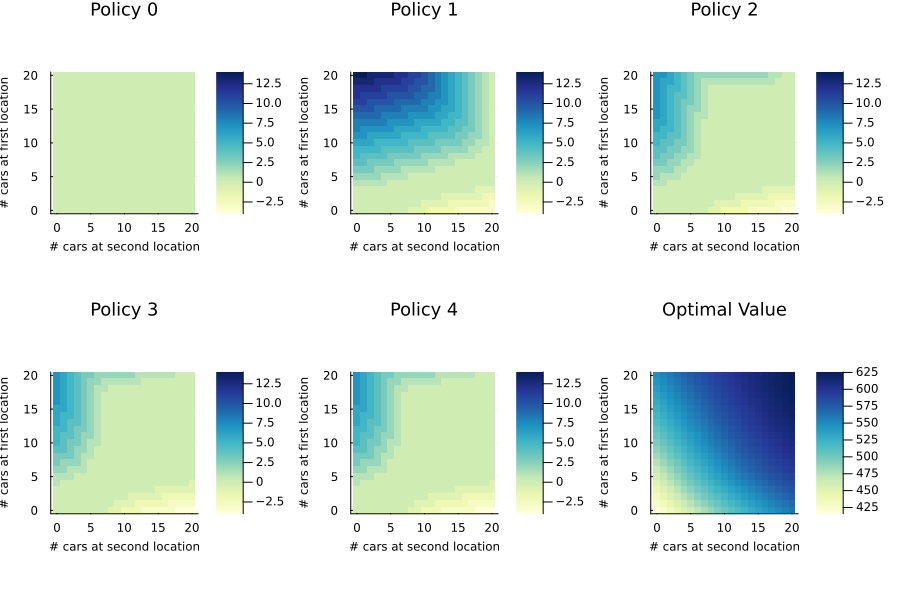
\includegraphics[width=11cm]{car_rental_policy_iteration_const.png}
\end{frame}

\begin{frame}{Car Rentals (Stochastic)}
	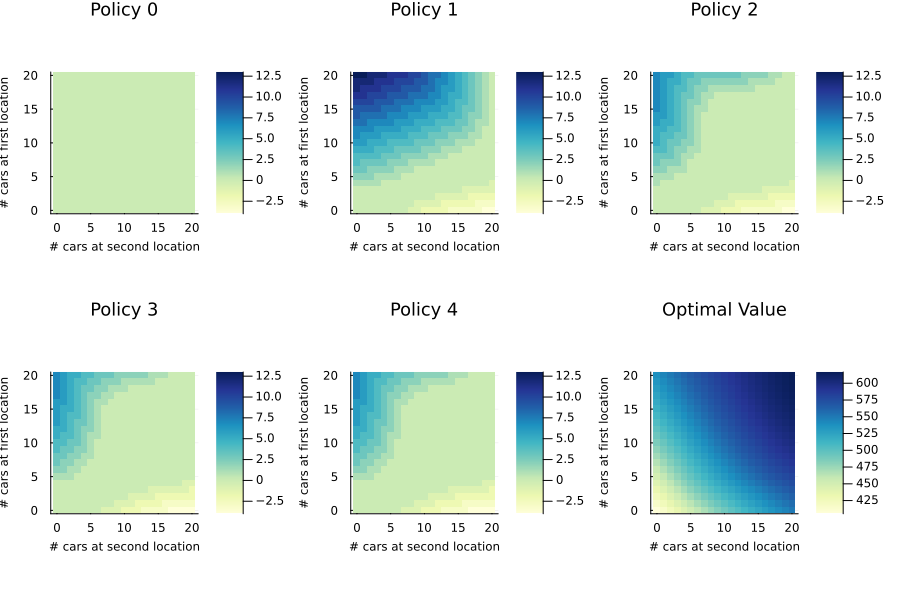
\includegraphics[width=11cm]{car_rental_policy_iteration_stoch.png}
\end{frame}

\begin{frame}{Gambler's Problem Value ($p = 0.4$)}
	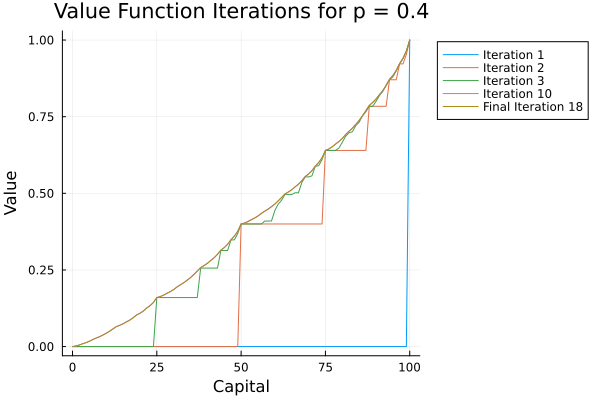
\includegraphics[width=11cm]{gamblers_problem_value_p04.png}
\end{frame}
\begin{frame}{Gambler's Problem Policy ($p = 0.4$)}
	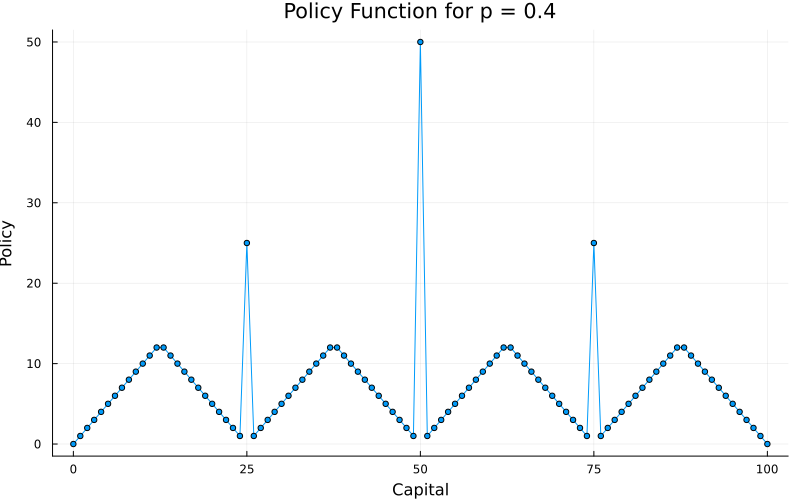
\includegraphics[width=11cm]{gamblers_problem_policy_p04.png}
\end{frame}
\begin{frame}{Gambler's Problem Value ($p = 0.25$)}
	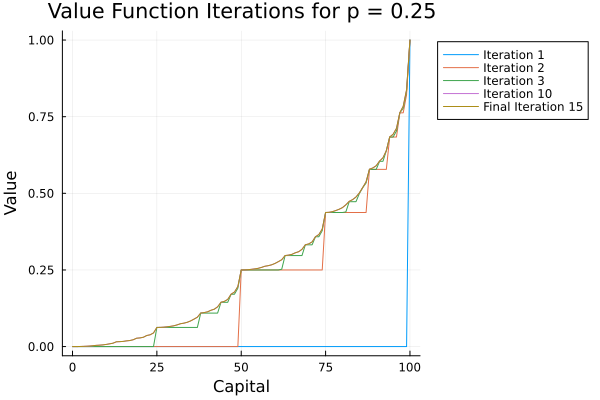
\includegraphics[width=11cm]{gamblers_problem_value_p025.png}
\end{frame}
\begin{frame}{Gambler's Problem Policy ($p = 0.25$)}
	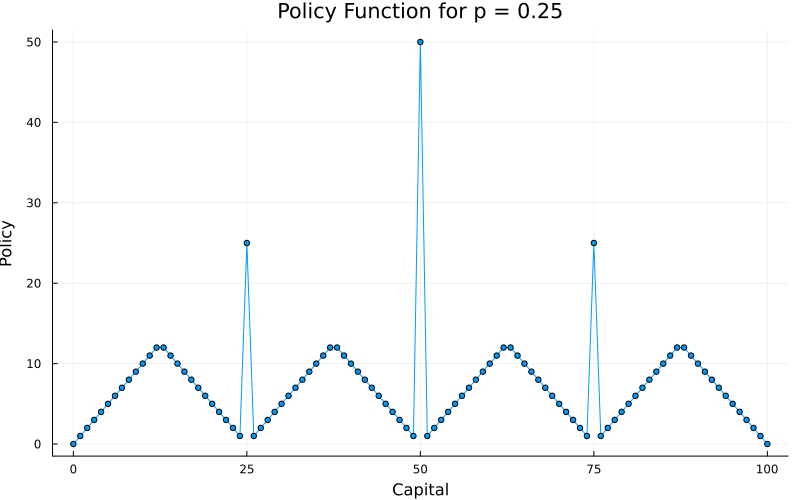
\includegraphics[width=11cm]{gamblers_problem_policy_p025.png}
\end{frame}
\begin{frame}{Gambler's Problem Value ($p = 0.55$)}
	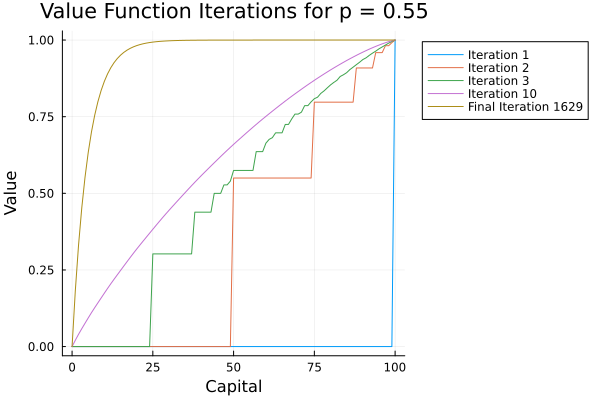
\includegraphics[width=11cm]{gamblers_problem_value_p055.png}
\end{frame}
\begin{frame}{Gambler's Problem Policy ($p = 0.55$)}
	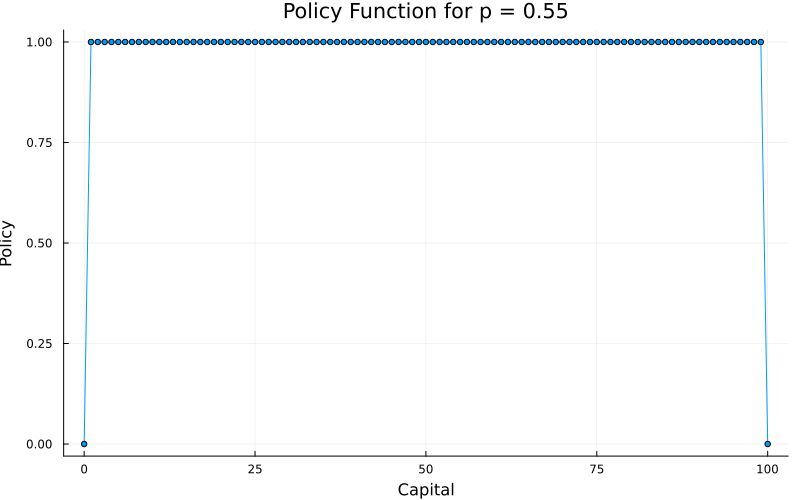
\includegraphics[width=11cm]{gamblers_problem_policy_p055.png}
\end{frame}
\begin{frame}{Gambler's Problem Value ($p = 0.75$)}
	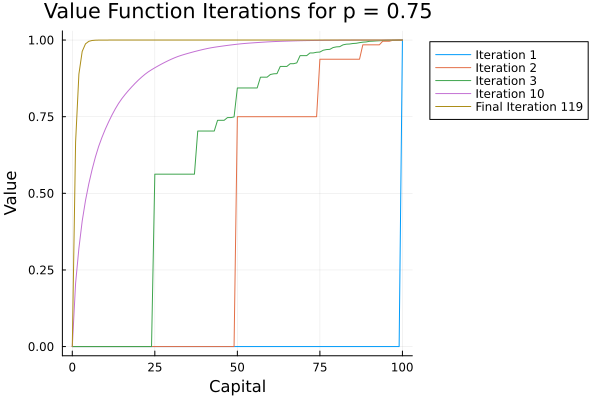
\includegraphics[width=11cm]{gamblers_problem_value_p075.png}
\end{frame}
\begin{frame}{Gambler's Problem Policy ($p = 0.75$)}
	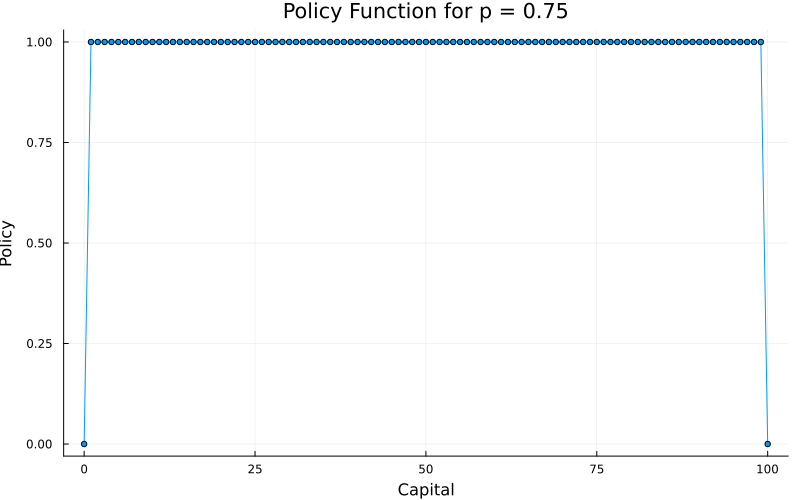
\includegraphics[width=11cm]{gamblers_problem_policy_p075.png}
\end{frame}

\end{document}













